\documentclass{article}

\usepackage{amsmath}
\usepackage{graphicx}

\begin{document}

\section{Introduction}

Fishery managers have only one ``lever" to pull when it comes to fishery management: the ability to set harvest quotas.  Fishermen work within these quotas by exerting various levels of fishing effort.  Both managers and fisherman can better understand the ecosystem they work within and the implications of their decisions with the assistance of a production model, which is a system of differential equations designed to predict outcomes.  A visualization enhances such a model by making its inner workings more explicit. We hope to show that our visualization of the MS-PROD model is valuable tool to the modellers and stakeholders alike. 

\section{Background}

\subsection{The Model}

Both the short- and long-term effects of human exploitation on an ecosystem such as a fishery are not easily understood.  Experiments which would allow ecosystem managers to investigate the impact of different levels of exploitation over many years would be either impractical or impossible to conduct on a large scale.  Fortunately, ecosystem models can be used instead to help gain a better understanding of an ecosystem.

Ecosystem models are abstract representations of an ecological system, which could mean anything from an individual species to an entire community of species.  A classic example is the Lotka-Volterra model, which is a pair of differential equations for describing the non-linear interactions between a predator species and a prey species. \cite{Lotka1926fds, VOL26a}:

\begin{align}
   \frac{d x_1}{dt} &=   x_1 \left(\alpha - \beta  x_2\right) 
\\ \frac{d x_2}{dt} &= - x_2 \left(\gamma - \delta x_1\right)
\end{align}
where $x_1$ is the number of prey, $x_2$ is the number of predator, $t$ is time, $\alpha$ is the prey's growth rate, $\beta$ is the rate at which the predator destroys the prey, $\gamma$ is the death rate of the predator, and $\delta$ is the rate at which the predator increases from consuming the prey.  The model can be generalized to discuss an arbitrary number of species rather than just a single pair.

The Lotka-Volterra model can be modified to take competition instead of predation into account, as in the Rosenzweig-MacArthur model \cite{Rosenzweig1963Graphical} and the Leslie-Gower model \cite{leslie1960}.  These adaptations to the model also consider carrying capacity, which is the maximum number of a species that can sustained indefinitely:

\begin{align}
   \frac{d x_1}{dt} &= r_1 x_1 \left(1 - \left(\frac{x_1 + \alpha_{12} x_2}{K_1}\right)\right)
\\ \frac{d x_2}{dt} &= r_2 x_2 \left(1 - \left(\frac{x_2 + \alpha_{21} x_1}{K_2}\right)\right)
\end{align}
where $r_i$ is the growth rate for species $i$, $K_i$ is the carrying capacity for species $i$, and $\alpha_{ij}$ is the effect species $j$ has on species $i$.  As with Lotka-Volterra, this model concerns only two species, but it can be generalized to include more than two.

Both Lotka-Volterra and Leslie-Gower do not incorporate a factor which is critical when discussing fisheries management: the effect of harvest.  For this, the Schaefer model is most often used \cite{schaefer1957}:

\begin{align}
   \frac{d x}{dt} &= r x \left(1 - \left(\frac{x}{K}\right)\right) - q E N
\end{align}
where $r$ is the growth rate, $K$ is the carrying capacity, $q$ is the catchability coefficient, and $E$ is the fishing effort.

Simple models, when available and correct, are appreciated; since fewer components are needed to describe their real-world counterparts, they are more easily understood and implemented.  All three of these models are subjectively simple in that they only consider a few ecological factors each. However, ecosystems are complex systems which require management that recognizes them as such \cite{Christensen1996Report}.  Thus, a more holistic approach called ecosystem-based fishery management (EBFM) has been advocated \cite{united1999ecosystem}.  However, this approach has not often been implemented due to a lack of models which consider all necessary ecological factors.  Gamble and Link developed a multispecies production model (MS-PROD) to fill this gap \cite{Gamble20092570}.

The MS-PROD model is built upon the Schaefer production model by also including Lotka-Volterra terms for predation, Leslie-Gower terms for competition, and carrying capacities for functional groups ($K_G$) as well as for the entire system ($K_{\sigma}$):

\begin{align}
\frac{d N_i}{dt} &= r_i N_i \left(1 - \frac{N_i}{K_G} - \frac{\displaystyle\sum\limits_{j=1}^g \beta_{ij} N_j}{K_G} - \frac{\displaystyle\sum\limits_{j=1}^G \beta_{ij} N_j}{K_{\sigma} - K_G}\right) - N_i \displaystyle\sum\limits_{j=1}^P \alpha_{ij} N_j - H_i N_i
\end{align}
where $N_i$ is the number (or biomass) of species $i$, $t$ is a unit of time, $r_i$ is growth rate for species $i$, $\beta_{ij}$ is the interaction of species $j$ on $i$, $\alpha_{ij}$ is the predation of species $j$ on $i$, $H_i$ is the harvest rate on species $i$, $g$ is the number of species within species $i$'s group, $G$ is the number of groups, and $p$ is the number of predators.

This model is distinguished from other multispecies production models by describing stocks with explicit ecological and harvest factors.  Ten key species were chosen from the Northeast United States Continental Shelf Large Marine Ecosystem (NEUS LME) from four major functional groups.  Given input parameter set of initial biomass values, a predation matrix, an interaction matrix, catchability values, and harvest effort values, the MS-PROD model runs simulations for 30 years with an annual time step to predict individual biomasses.  While this outputted information is potentially valuable to fishery managers, it was lacking an interactive graphical user interface.  

\subsection{Visualization Methods}

Fisheries management is focused on the sustainability of choices concerning fish stocks.  A main purpose of ecosystem management is to ensure future generations can enjoy the same natural resources \cite{Christensen1996Report}.  Thus, fisheries management is a time-oriented discussion.  As such, the MS-PROD model provides biomass forecasts for 30 years.  Therefore, time-oriented visualization techniques must be explored.

Frank discusses the different types of time-oriented data by defining three criteria: a) linear vs. cyclic, b) time points vs. time intervals, and c) ordered time vs. branching time vs. time with multiple perspectives \cite{frank98times}.  The MS-PROD data consist of discrete time points with definite starting and ending points, falling under the linear time and time points categories.  As for the third criterion, the model outputs one ordered time result for a single execution, however fisheries managers may like to compare alternative scenarios.  Therefore, our domain falls into the branching time category.  Aigner et al. point out that techniques for visualizing branching time and time with multiple perspectives are unfortunately less common \cite{Aigner08visualmethods}, but a common technique for ordered time such as a line chart serves as a good starting point.

\begin{figure}[htb]
	\centering
	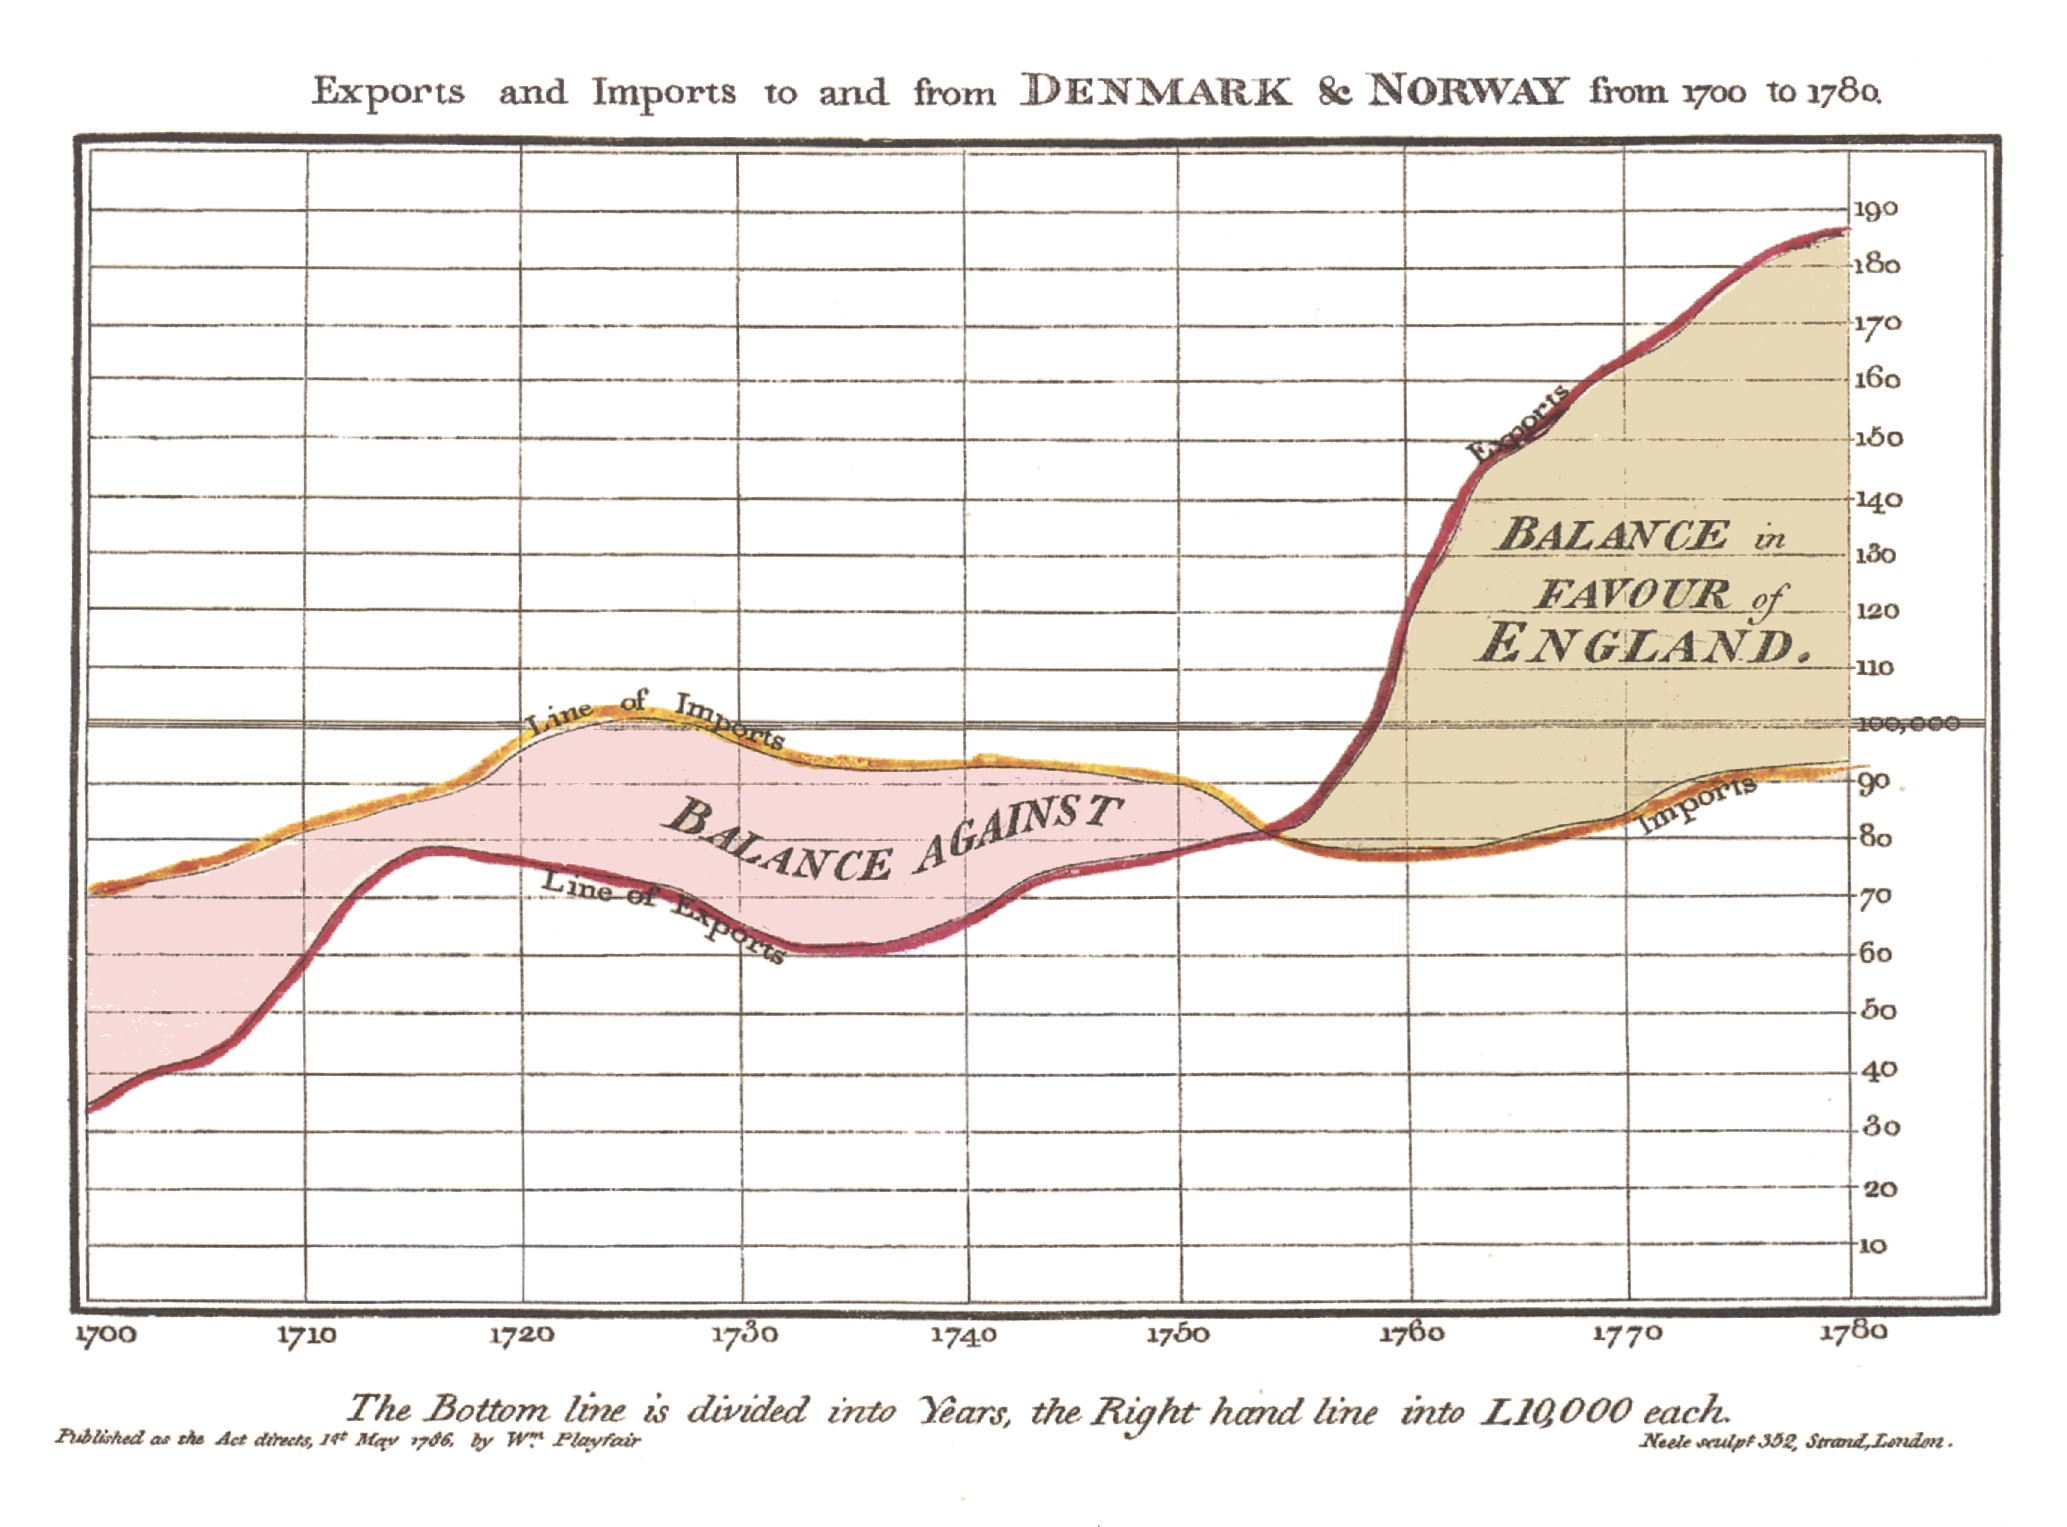
\includegraphics[width=10cm]{figures/PlayfairTimeSeries.eps}
	\caption{Playfair's original time series chart \cite{playfair}.}
	\label{fig:playfair}
\end{figure}

The line chart was first invented by William Playfair in 1786 to communicate time series data, seen in Figure~\ref{fig:playfair} \cite{playfair}.  Today, it remains a common method for visualizing time-oriented data in many fields, including science, economics, planning, and engineering to name a few.  Line charts typically encode time on the horizontal axis, progressing from left to right, and some time-varying value on the vertical axis.  Points in the chart are connected by line segments such that the slope of the line indicates the rate of change between time steps.  There has been much research done on the effectiveness of time series in various forms, which helps to make decisions regarding our visualization of MS-PROD.

%\subsection{The Model}

%Both the direct and indirect effects of harvests on the various fish populations are not easily understood, especially over time.  The growth or decline of one species can easily affect other species in the ecosystem.  The MS-PROD and Kraken models were created using genetic algorithms fitted to historical data to describe population sizes in terms of harvest, predation, competition, and interaction.

%Though these models are useful tools, a more sophisticated interface is necessary to aid in users' understanding of the effects of the various input parameters.  This interface will aid in the comparision of key individual species as well as functional groups.  Part of the interface will include a collection of time series plots representing the modeled biomass of different fish populations over time.  Users will be able to interactively investigate the impact of different levels of effort from fishermen on these populations by controlling effort with sliders, which will result in new time series plots.  Another part of the interface will include network visualizations for the predation, competition, and harvest terms, which would help to illustrate to users which relationships are significant according to the models.  

%Many expansions upon the original models are being considered as well, which will be included in the interface and visualization, such as separate levels of effort for the different types of fishing fleets.  The models aim to provide insight into historical fish population sizes and ultimately to estimate the future size of stocks.  Coupled with a well-designed interface, these models will give managers advice on estimated stock levels, which would in turn help them to recommend fishing quotas.

%\subsection{Previous Work}

%Tweedie et al. developed the Influence Explorer, which is an interface for understanding the relationships between different attributes in a design process \cite{conf/chi/TweedieSDS95}.  Parameters values are randomly selected to represent different possible items.  For each attribute, there is a histogram including each of the items.  The attribute ranges are controlled by sliders.  When the user adjusts the slider of a given attribute, all items that are within that range are highlighted on all of the histograms.  Industrial designers found the ability to interactively explore the effects of different parameter ranges to be valuable.

%Ferreira et al. created the BirdVis, a visualization of a statistical model for predicting bird distribution across time and space \cite{Ferreira:6065004}.

%Javed et al. studied the merits of different plotting techniques for multiple time series \cite{Javed:2010:GPM:1907651.1907971}.  Their user study revealed that a simple line graph with all time series on one plot or a single graph for each time series is better suited to different tasks than a horizon graph or a braided graph.  They also found that users complete tasks more correctly when there is more display space allocated to the graphs.  A higher number of time series is discouraged because it also leads to a decline in correct task completion.

%Knuth illustrated interaction of characters in Victor Hugo's novel \textit{Les Mis\'erables} with an arc diagram \cite{Knuth:1993:SGP:164984}.  Each character is represented with a circular node, where size indicates the number of appearances.  The nodes are arranged linearly, colored and ordered according to clusters of characters that appear together frequently.  Semi-transparent arcs are drawn between the characters which appear in the same chapter, with the thickness of the arc representing the number of such appearances.  %Smaller datasets which contain particular clusters of nodes are well suited to arc diagrams. 

%Holten and van Wijk studied the effectiveness of different techniques for indicating directionality of edges in a graph \cite{Holten:2009:USV:1518701.1519054}.  The traditional arrowhead was compared with other representations of direction and was found to perform poorly.  One of their recommendations was that a dark-to-light representation is clearer than light-to-dark for an intensity-based direction cue.

%Wattenberg developed the arc diagram to illustrate repeated sequences in strings or music \cite{Wattenberg:2002:ADV:857191.857733}.  The arc diagram represents the units or significant units of the sequence as nodes that are arranged chronologically in a line.  A translucent arc is drawn between identical units, where the width of the arc corresponds to the length of the repeated sequence, to give a clear indication of pattern and repetition.  Others 

\bibliographystyle{plain}

\bibliography{thesis}

\end{document}


